\section{Nebulas Force}
\label{sec:nebulasforce}

We use Nebulas Force (NF) to describe the evolving capability of the blockchain system and its applications. As the first driving force of the blockchain system and its application development, the Nebulas Force includes three aspects, that is, the Nebulas Virtual Machine (NVM), the upgrade of the protocol code in the blockchain system, and the upgrade of the smart contract running on the blockchain system.

%我们使用星云原力(Nebulas Force, NF)来描述区块链系统及应用的进化能力。星云原力做为驱动区块链系统及应用发展的第一推动力,包括三个方面:星云链虚拟机NVM(Nebulas Virtual Machine),区块链系统中核心协议的升级,以及运行在区块链系统之上的智能合约的升级。

In Nebulas, we will introduce LLVM to implement the Nebulas Virtual Machine (NVM). The protocol code and the smart contract code will be compiled into NVM bytecode, which is dynamically compiled and optimized with the LLVM just-in-time (JIT) compilation function and eventually executed in the sandbox environment. Meanwhile, with the modular architecture of LLVM, developers can use their familiar programming languages to implement safer and higher-performance smart contracts, providing users with various decentralized applications.

%在星云链中,我们将引入LLVM来实现星云链虚拟机NVM。核心协议和智能合约代码将会编译成NVM字节码,通过LLVM即时编译(Just-in-time compilation)功能,实现其动态编译和优化,最终在沙箱环境中执行。同时借助于LLVM的模块化架构,开发者可以用熟悉的编程语言实现更高性能和更安全的智能合约,给用户带来更丰富的去中心化应用。

For the upgrade of the protocol code in Nebulas, Nebulas will add the protocol code to block structure to carry out the upgrade of the protocol code by supplementing additional data on chains so as to avoid the possible split or bifurcation between developers and communities. With the development of Nebulas communities, the upgrade capability of NF and basic protocols will be gradually open to communities, and communities will define the evolving direction of the Nebulas and achieve its upgrade target. With the help of the core technology and the opening concept of NF, Nebulas will have a continuously evolving space and an infinitely evolving possibility. For example, a series of parameters including the NR algorithm parameter, the PoD incentive amount, the consensus algorithm and the production rate of new tokens can be gradually adjusted during the development of Nebulas without upgrading most client codes.

%对于星云链中的核心协议升级,星云链将核心协议加入到区块中,通过对链上数据的追加实现核心协议的升级,避免开发者和社区的分裂或分叉的可能性。随着星云链社区的发展,NF及基础协议升级能力将逐步开放给社区,由社区定义星云链的进化方向并实现其升级目标。借助于NF这个核心技术和开放性的理念,星云链将会具有持续的进化空间和无限的进化可能。例如,NR算法参数、PoD激励金额、共识算法及新代币的生产速度等一系列参数,都可以在星云链的发展过程中逐渐调整,而不需要大部分客户端代码的升级。

The smart contract is usually considered to be permanent and does not support upgrading. With the help of the design of underlying storage of the smart contract to support the cross-contract visit of state variables, Nebulas can complete the upgrade of the smart contract. This solution is very friendly to developers, making them respond to bugs more rapidly, which can prevent huge losses to users caused by any hacker events.

%智能合约通常被认为是永久性的,不支持升级。星云链通过在智能合约底层存储支持状态变量可跨合约访问的设计,完成智能合约的升级,这种解决方案对开发者友好,使得开发者面对漏洞,能够更快的响应和升级,避免黑客事件给用户带来巨大的损失。

\subsection{NVM 星云链虚拟机}
\label{sec:nvm}

我们将引入LLVM~\cite{llvm}做为NVM的核心组件,并使用LLVM Byte Code做为NVM字节码。NVM字节码通过LLVM JIT完成动态编译和优化,运行在NVM沙盒环境中。在这种架构设计下,星云链的核心代码、智能合约能直接享受到LLVM带来的性能和安全性的不断提升。

LLVM早期是Low Level Virtual
Machine的缩写,是一系列高度模块化的编译器和工具链技术的集合,包括Google、Apple在内的公司都使用它做为代码编译框架。LLVM提供了一套中立的中间表示(LLVM
IR)和相应的编译基础设施,并围绕这些设施提供了一套全新的编译策略,包括对LLVM
IR的优化、LLVM IR到不同硬件平台的代码生成、LLVM IR到LLVM Byte
Code的代码生成以及LLVM Byte Code在不同硬件平台上通过LLVM
JIT直接执行。如图\ref{fig:llvm}所示

%LLVM编译框架分为三层,第一层支持多种语言作为输入(例如C/C++,go和python等),第二层是一个共享式的优化器(对LLVM IR做优化处理),第三层是许多不同的目标平台(例如 Intel, ARM和PowerPC),如图\ref{fig:llvm}所示

\begin{figure}[h]
\centering
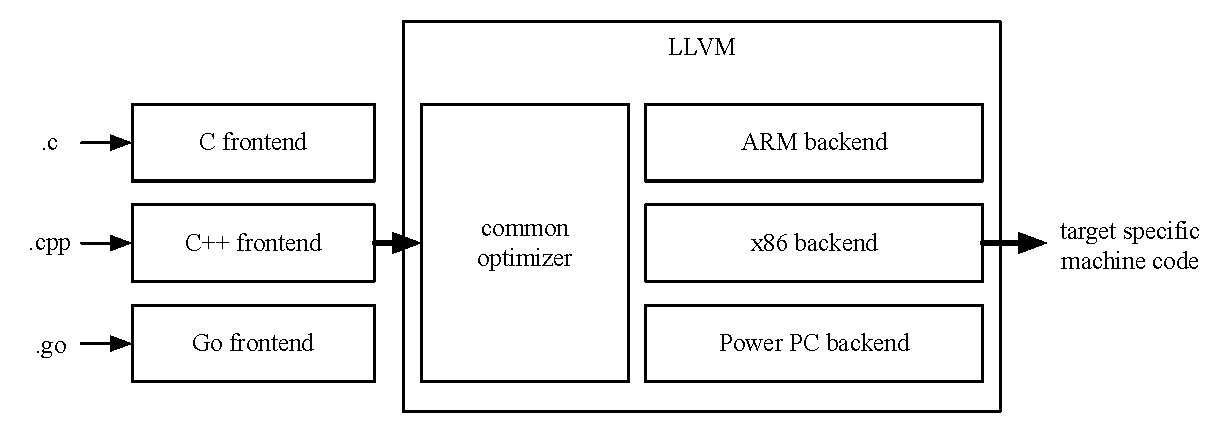
\includegraphics[width=10cm]{./figs/llvm}
\caption{LLVM}
\label{fig:llvm}
\end{figure}

我们依托LLVM构建NVM,如图\ref{fig:nvm}所示。首先,我们提供区块链底层API库;然后,我们为不同语言(如Solidity,JavaScript
,C/C++,Go等)构建生成LLVM
IR的编译器前端;最后,利用LLVM提供的工具链,生成LLVM Byte Code。最终,LLVM Byte
Code通过LLVM的JIT引擎运行在NVM提供的安全的沙箱环境中。
%然后,利用LLVM链接器链接我们提供的底层库,LLVM
%JIT完成核心协议和智能合约代码的编译、优化以及跨平台适配,生成机器代码;最后,让这些机器代码通过LLVM的JIT引擎运行在NVM提供的安全的沙箱环境中。

\begin{figure}[h]
\centering
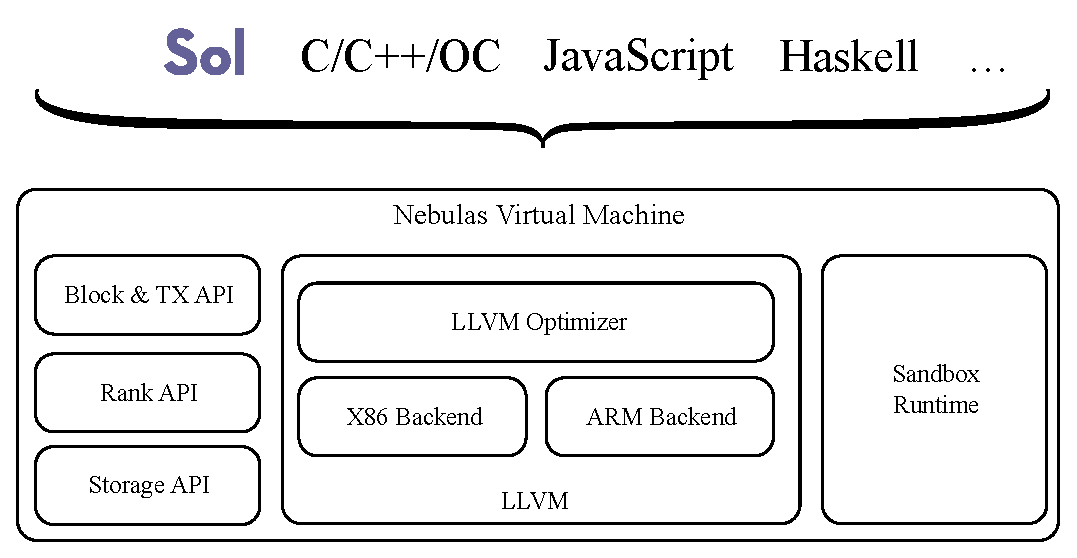
\includegraphics[width=10cm]{./figs/nvm}
\caption{星云链虚拟机}
\label{fig:nvm}
\end{figure}

NVM是星云原力的重要基石。新的协议代码或智能合约发布时,NVM中LLVM编译器模块完成新代码的编译得到LLVM字节码,然后发布到链上;链上确认后,新代码将由LLVM
JIT完成编译和优化,然后进入沙箱取代旧代码并被执行,过程如图\ref{fig:nvm-process}所示。 \\

\begin{figure}[h]
\centering
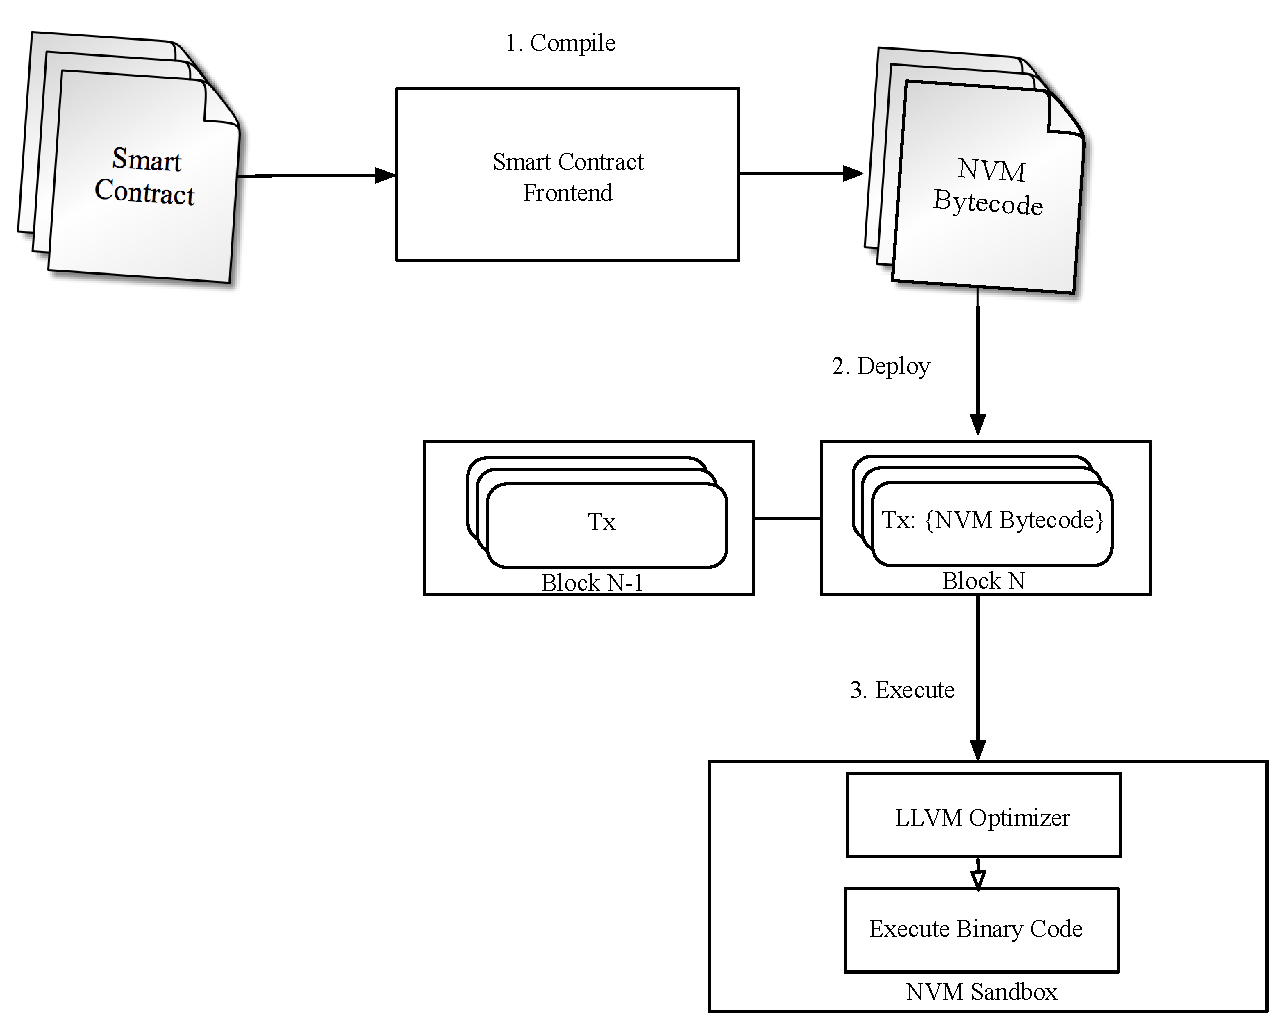
\includegraphics[width=10cm]{./figs/nvm-process}
\caption{星云链虚拟机运行机制}
\label{fig:nvm-process}
\end{figure}

借助于LLVM(见\ref{fig:llvm}),NVM还支持开发者用其熟悉的编程语言开发智能合约和应用,比如以太坊智能合约所使用的Solidity,更加灵活的JavaScript,甚至是纯函数式语言Haskell。除了这些通用语言外,NVM还可以为不同领域和场景提供定制的高级语言,比如面向金融行业的DSL(领域专有语言)。这类高级语言面向行业、场景高度定制,使得它们更容易被形式化验证,能进一步提高代码健壮性和安全性,更有利于星云链开发者开发出更丰富的智能合约及应用。

\subsection{核心协议的升级设计}

我们首先给出星云链中的区块结构,然后讨论如何在该区块结构上实现核心协议的升级问题。

\paragraph{区块结构}

星云链区块数据结构包含,但不限于以下信息:
\begin{itemize}
	\item Header:区块头
		\begin{itemize}
		\item Height:高度
		\item ParentHash:父区块哈希值
		\item Ts:时间戳
		\item Miner:记账人地址
		\item Dynasty:区块所处共识朝代
		\item Epoch:区块所处共识时代
		\item RankVer:区块所处NR周期
		\item RankRoot:区块所处NR周期的排名哈希值
		\item StateRoot:状态根哈希值
		\item TxsRoot:交易根哈希值
		\item ReceiptsRoot:交易收据根哈希值
		\item TransNum:交易数
		\end{itemize}
	\item Transactions:交易数据(包含多个交易)
		\begin{itemize}
		\item From:交易发起人地址
		\item To:交易接收人(普通用户或智能合约)地址,对于创建智能合约,值为0地址
		\item Value:转账金额
		\item Data:交易的payload。如果交易为创建智能合约,则为智能合约字节码;如果交易为智能合约调用,包含调用函数名称和入参值
		\item Signature:交易签名
		\item Gas:燃料上限
		\item GasPrice:燃料单价
		\item Nonce:标识交易唯一性
		\end{itemize}
	\item Votes:Prepare和Commit票数统计(包含多个),用在PoD(见\refsec{sec:pod})共识算法中
		\begin{itemize}
		\item From:投票人
		\item VoteHash:投票区块哈希
		\item Hv:投票区块所处高度
		\item Hvs:投票区块的某祖先高度
		\item VoteType:投票类型,Prepare或Commit
		\item Signature:投票签名
		\end{itemize}
	\item Protocol Code:核心协议代码(一个区块中只能有0或1个)
		\begin{itemize}
		\item Hash:哈希值
		\item Code:核心协议的字节码
		\item ValidStartBlock:协议生效起始区块号
		\item Signature:签名(校验是否来自开发者社区保留账号的签名)
		\item Version:标识核心协议版本号,每次升级都需要递增,防止恶意记账人回滚到老的Protocol Code
		\item Nonce:标识唯一性
		\end{itemize}
	\item Nebulas Rank:星云指数(计算周期为一周一次,大部分区块没有)
		\begin{itemize}
		\item Address:账号地址标记
		\item Score:NR值
		\end{itemize}
\end{itemize}

\begin{figure}[h]
\centering
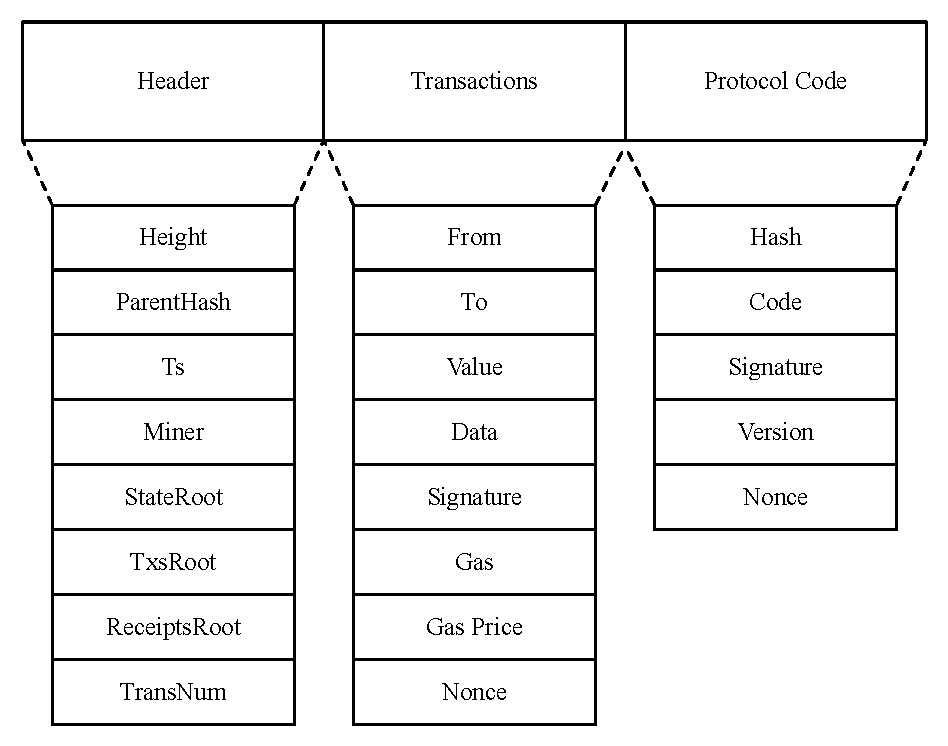
\includegraphics[width=13cm]{./figs/block}
\caption{区块结构}
\label{fig:block}
\end{figure}


类似于其他加密数字货币系统,用户和区块链上的互动都是通过特定的交易进行的。用户创建一笔交易,用自己的私钥签名后,发到区块链的任何一个节点中,通过P2P网络广播到全网节点。在固定的出块时间间隔内,由PoD共识算法(见\refsec{sec:pod})指定的记账节点累计这段时间内的所有交易,打包成标准格式的区块,同步到全网所有节点。经各节点独立验证后,加入本地账本,成为全球总账本的一部分。

以太坊中,交易分为两种类型:普通账户交易,智能合约交易。我们在星云链的区块中,增加新的数据类型:核心协议代码和星云指数。核心协议代码作为区块链数据的一部分存储在链上,星云链基础协议的升级,是通过链上数据的追加而实现的。星云指数根据NR排序算法,计算出每个周期各个账户的NR值存到链上,方便NR值的实时调用和历史排名查询。

\paragraph{核心协议的升级}

星云链客户端节点从当前最新区块的Protocol Code存储区可以取到编译后的虚拟机字节码(LLVM IR),如果当前最新区块没有Protocol Code数据,说明核心协议没有变更,就往前追溯到最近区块的Protocol Code。区块链的核心协议行为都由Protocol Code确定,包括验证算法、打包规则、NR算法、奖励机制等,几乎绝大部分的区块链行为都可以由Protocol Code定义。

如果核心协议需要升级,由星云链团队开发,把代码在公开渠道让社区讨论和投票。投票可以通过智能合约或者论坛投票的形式进行,当绝大部分社区成员都同意协议升级,星云链开发组把最新代码打包成Protocol Code交易,发布到全网节点,记账节点只要把其包含进区块,就可以在指定区块高度开始生效。这种方式的区块链协议升级,对客户端来说是透明的,无需软、硬分叉。

为了保证核心协议代码是经过授权发布的,Protocol Code的发布者是星云链核心开发组保留地址,该地址在创世区块内部硬编码无法变更。所有记账节点都会验证Protocol Code签名,签名不通过的视为非法数据。

后续的改进措施是把Protocol Code的签名校验改成M-of-N的多签名形式,这个本身也可以通过Protocol Code的升级实现。

\section{智能合约}

\subsection{图灵完备的智能合约编程语言}
智能合约是一套以数字形式定义的承诺(promises),包括合约参与方可以在上面执行这些承诺的协议。在物理上,智能合约的载体是计算机可识别并运行的计算机代码。比特币脚本语言是一种命令式的、基于栈的编程语言,由于它是非图灵完备的,所以应用上有一定的局限性。以太坊是全世界第一个实现图灵完备的智能合约的区块链系统,编程语言是Solidity、Surpent,使得应用开发者们可以高效快速地开发各式各样的应用程序。智能合约代码发布到区块链上之后,能够无需中介的参与,在区块链上自动执行。星云链中的智能合约编程语言,在初期时完全兼容以太坊的Solidity,方便开发者为以太坊开发的智能合约应用无缝的迁移到星云链中来。我们在Solidity语言中增加一些跟Nebulas Rank相关的指令集,方便开发者获取任意用户的NR值。后续我们会设计自己的智能合约二进制规范,推出各种编程语言的支持,使得开发者可以用自己喜欢的高级语言编程,例如Java、Python、Go、JavaScript、Scala等。

\subsection{合约可升级设计}
目前以太坊智能合约的设计是代码一经部署,不可变化,代码逻辑从部署的时刻起,便永远不再具有升级的能力。智能合约如果作为协议来看,不可变化是其要求的,代表着一种协议的约定,运行行为都是确定性的。但是随着智能合约开始获得越来越多的使用,其流程和代码也变得越来越复杂,人们发现,就像现实世界的合同一样,如果没有认真审核的话,在设计和编码过程中难以避免人工失误的产生,一旦被黑客找到漏洞,损失往往是巨大的。2016年6月,The DAO攻击事件,由于一个代码缺陷,导致以太坊用户损失了共计6000万美元的损失;最近Parity钱包的漏洞,导致15万个以太币的流失,价值3000万美元。比特币由于其设计上的非图灵完备性,删减了许多脚本指令,所以其安全性是极高的。

虽然目前有各种智能合约编程的最佳实践,以及更严格的审核流程,甚至出现形式化验证工具,通过数学证明的方式验证智能合约的确定性。但是既然是代码,就不可能没有漏洞。回顾我们现在的中心化的互联网世界,各种互联网服务都是可以升级的,弥补开发过程中发生的各种漏洞。任何一个完美的应用系统,都是演化而不是设计出来的。我们认为,解决智能合约安全性的根本问题,需要有一个好的智能合约可升级设计方案。

以太坊上的智能合约可升级设计有一些解决方案,大体上分为两类:一类是对外公开proxy contract(代理合约),代理合约的代码非常简单,仅仅把请求转发给后面的真正的功能合约。当需要升级合约时,把代理合约的内部功能合约指针指向新的合约即可;第二类是把合约的代码和存储分离,存储合约负责提供方法,供外部合约读写内部状态,代码合约做真正的业务逻辑,升级时只需要部署新的代码合约,不丢失所有的状态。这两类方案都有其局限性,不能解决所有问题:合约的代码和存储分离在设计上增加了很多复杂度,有时候甚至不可行;代理合约虽然能够指向新合约,但是老合约的状态数据并不能迁移;有些合约在开始开发时,没有良好的设计,没有为以后的升级留下接口。

我们设计一种简洁的智能合约升级方案:在语言层面上,我们支持一个合约的状态变量供另外一个合约直接读写(符合安全约束)。这是一个例子,假如有个Token合约,代码如下:
\begin{lstlisting}[frame=single]
contract Token {
  mapping (address => uint256) balances shared;

  function transfer(address _to, uint256 _value) returns (bool success) {
     if (balances[msg.sender] >= _value) {
       balances[msg.sender] -= _value;
       balances[_to] += _value;
       return true;
     } else {
       return false;
     }
   }
   function balanceOf(address _owner) constant returns (uint256 balance) {
       return balances[_owner];
   }
}
\end{lstlisting}

合约部署时,balances变量用关键字shared标识,编译成字节码运行时,虚拟机会为该变量单独设计存储区域。不用关键字shared声明的变量,都不可以被其它合约直接访问。

假如原代码的transfer函数需要修改一个bug,对\_value做检查,部署新的智能合约代码:

\begin{lstlisting}[frame=single]
[baseContractAddress="0x5d65d971895edc438f465c17db6992698a52318d"]
//baseContractAddress是老合约的地址
contract Token {
  mapping (address => uint256) balances shared;

  function transfer(address _to, uint256 _value) returns (bool success) {
     if (balances[msg.sender] >= _value && _value > 0) {
       balances[msg.sender] -= _value;
       balances[_to] += _value;
       return true;
     } else {
       return false;
     }
   }
   function balanceOf(address _owner) constant returns (uint256 balance) {
       return balances[_owner];
   }
}
\end{lstlisting}

新的合约部署以后,老的合约可以选择selfdestruct,不能再被访问,但是shared变量依然被永久保留。新的合约可以完全继承老合约的balances资产,全部的状态都不丢失,不需要做额外的迁移工作。但是在开发智能合约时,对关键的状态变量声明为shared是必须的,编译器会对变量的存储区域做特殊处理,保证其可以被其它授权的合约访问。

为了保证安全,升级合约和老合约必须是相同的creator,否则运行时会抛异常。

这种设计存在道德上的问题,因为合约的内容条款一旦拟订,其实是不应该被修改的,至少修改必须征询合约受众的同意。我们计划引入投票机制,以批准智能合约的升级,而不是默默的被合约创建者修改。

通过这种可升级方案,The DAO或者Parity类似的漏洞攻击事件,可以更快的被修复,而不是通过硬分叉的方式。并且修复以后,所有用户的资产都不需要迁移,仍然继续使用。



